%%%%%%%%%%%%%%%%%%%%%%%%%%%%%%%%%%%%%%%%%%%%%%%%%%%%%%%%%%%%%%%%%%%%%%%%%%%%%%%%

% IEEEconf.cls file must exist in the same directory as the TeX file you want to compile
\documentclass[letterpaper, 10 pt, conference]{IEEEconf}

\title{\LARGE \bf
COMPUTER HISTORY\\
\large Computer Games Expressed In A Few Words
}

\author{Group Number 3\\
\small Ambrosia Ingoglia\\
\small Alyssa Daniel-Peterson\\
\small Quoya Gable-Lairsey\\
}

% Image/graphics support
\usepackage{graphicx}
\graphicspath{ {./images/} }

% Formatting for lists
\usepackage{enumitem}

% Formatting for media
\usepackage{float}
\restylefloat{table}
\restylefloat{figure}

\begin{document}


\maketitle
\thispagestyle{empty}
\pagestyle{empty}

%%%%%%%%%%%%%%%%%%%%%%%%%%%%%%%%%%%%%%%%%%%%%%%%%%%%%%%%%%%%%%%%%%%%%%%%%%%%%%%%
\section{INTRODUCTION}

The technological advancement of computers in the 20th century has led to people finding new ways of having fun. Entertainment is a pastime as ancient as time and one  that everyone partakes in. Playing games on computers hit a spike of popularity in the 60’s, as people all over the world began to expand the new medium of entertainment. By the 70’s the genre of entertainment began to hit the mainstream as pong was invented and by the 80’s it was difficult to meet someone who had never heard of it. Computer gaming is an amazing byproduct of Scientific genius, creativity and the want to be entertained.


%%%%%%%%%%%%%%%%%%%%%%%%%%%%%%%%%%%%%%%%%%%%%%%%%%%%%%%%%%%%%%%%%%%%%%%%%%%%%%%%
\section{TIME PERIOD}

Today, we find video games in households worldwide. Making up a 100 billion dollar global industry. With almost just as many games to choose from, available on many platforms, from console games to desktop. But today's games differ from where they started. Beginning in 1949, Donald Davis and his Naughts and Crosses Machine and in 1958 with William Higinbotham’s Tennis for two. They created both these games in labs learning more about the basics of computers through these gaming methods. Though all were very simplistic and didn’t have amazing graphics or even great visuals, it led to a lot bigger things like SpaceWars! which was released in 1961; it became huge and super inspiring to many young college kids, becoming the greatest thing of the time. SpaceWars! As created by students at MIT, the creators of the PDP asked them-1 to build an application for their computer to bring in some money. PDP-1 had a large display, a console typewriter, a tape reader and 9 kilobytes of computing ability. Through inspiration of the current exploration of space being a prominent thing in society, they developed an idea of applying it to spaceships. Which eventually developed into SpaceWars. This inspired many young programmers. Soon, bigger advancements quickly came. With the release of the Brown box and the development of Odyssey in 1972, video games through your TV now became official. Following Pong created by Atari, the first successful video game craze. Which built the foundation of the iconic 80s arcades, and the beginning of the video game golden age. 
In 1980, the release of Pac-Man, which became a pivotal moment for video games, as Pac-Man became a pop culture icon through the popularity the games brought. Much like modern games are today. Then with the development of graphics by Nintendo in 1985, they released the Famicom, with 18 game titles, with ionic games like Legend of Zelda, and the Super Mario Bros which are still relevant in today's pop culture. Soon followed by the Game Boy with its release in 1989. At this point technology is growing rapidly and computers are growing stronger with more capability than they would with the years before it. With more and more growth, with games like the sims, doom, tomb raider and many, many more. Starting the foundations of one of todays biggest video game company's today, Nintendo. All started with big cluncky machines like the PDP-1. The development of technology has been rapid and still very relevant to today and our modern pop culture.  

%%%%%%%%%%%%%%%%%%%%%%%%%%%%%%%%%%%%%%%%%%%%%%%%%%%%%%%%%%%%%%%%%%%%%%%%%%%%%%%%
\section{COMPUTER HARDWARE}

Tennis for Two is usually regarded as the oldest video game, depending on whom you ask. It was the first computer game made for entertainment rather than purely demonstration and research. This game was created by American physicist William Higinbotham, who originally wanted to create an interactive demonstration that would attract people’s interest during visitors’ days at his job. In 1958, Higinbotham got the idea for the game after reading an instruction manual for an analog computer. He found that it could find the wind resistance using a bouncing ball. Using an oscilloscope to display the game, Higinbotham quickly replicated a simple tennis simulation with two players. Players would turn a knob to adjust the angle of the ball and push a button to hit the ball towards the other player; it was impossible not to hit the ball, but there was a chance it would not go over the net due to a wrong time or angle. When the ball hit the ground, it had the same physics as a real tennis ball. A reset button was pressed to start the next round. This was Tennis for Two.

\begin{figure}[h!]
\centering
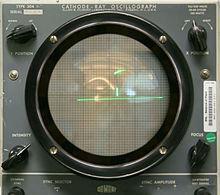
\includegraphics[width=0.5\textwidth]{tennis.jpg}
\caption{Tennis for Two on a DuMont Lab Oscilloscope Type 304-A}
\label{fig:example}
\end{figure} 

\ref{tbl:example} 
\begin{table}[h!]
\begin{center}
\scalebox{0.7}{
\begin{tabular}{||c | c | c | c||} 
\hline
  & Year Released & units sold & Today's net worth\\ [0.5ex]
\hline\hline
Tetris (game boy) & 1984 & 35 million  & 220 million) \\ 
\hline
Pac Man & 1980 & 10.44 million  & est. 510 million \\
\hline
Legend of Zelda & 1986 & 6.51 million & 40 million \\
\hline
Super Mario Bros & 1985 & 40.24 million & 30.25 billion\\
\end{tabular}
}
\caption{Popular 1980s video games and their current net worth}
\label{tbl:example}
\end{center}
\end{table}

\section{COMPUTER SOFTWARE}
Of course, Tennis for Two did not have fancy graphics like we have today. The cathode ray tube displayed a side view of a tennis court (which was simply two lines, one for the ground and one for the net). The ball itself was a dot that bounced back and forth on the screen, and players had to keep score themselves. Tennis for Two was very simple, primarily using resistors, capacitors, and relays. However, it did use transistors for the fast switching needed when the ball was in play. The display was five inches in diameter when it was first unveiled. A larger display screen was added. Also, he added another feature so that the game could simulate stronger or weaker gravity so that visitors could play tennis on the moon, for example. Tennis for Two was retired in 1960. The oscilloscope and computer were recycled for different uses, and Higinbotham worked on another display for visitors to enjoy.

\section{CONCLUSION}

Computer gaming is a genre like no other as it evolves constantly with no showings of stopping. At its earliest, William Higinbotham’s Tennis for Two, captivated audiences and spawned a genre because of it. This display of entertainment is something that has spurred many people's imaginations to create computerized experiences for people to enjoy. It's humble beginnings was a surprise and a major contradiction to what the gaming industry has become, what was once a interactive demonstration is now a billion dollar industry. Video games have taken the entertainment industry by storm, toppling both the music and film industry and giving rise to a cultural phenomenon. 

\section*{REFERENCES}

\begin{enumerate}[label={[\arabic*]}]
\item Computer History Museum. "Computer Games", Computer History, Accessed 23 October 2021,
https://www.computerhistory.org/revolution/computer-games/16/187
\item Oldest. "10 Oldest Video Games in the World", Oldest.org, Accessed 23 October 2021,
https://www.oldest.org/entertainment/video-games/
\item APS. "October 1958: Physicist Invents First Video Game", APS.org, Accessed 23 October 2021,
https://www.aps.org/publications/aps-news/200810/physicshistory.cfm
\item 

\end{enumerate}

\end{document}

